\section{modelling}

\emph{Note: }We denote a Layer in a general meaning by 'physical layer' 
or 'MAC layer' and our concrete C++ classes by \h{\bp} or \h{\bm}.

\subsection{overview}

Here we present the design- and interface details of the OMNeT-module 
\h{\bp} to meet the requirement specification. That includes:

\begin{enumerate}
 \item internal class diagram of \h{\bp} and relation to \h{\bm}
 \item interface description for all involved C++ classes
 \item flow charts for reception of MacPacket from upper layer and 
 AirFrame from the channel
 \item some detailed flow charts for important sub processes
\end{enumerate}


\subsection{classgraph}

We start with the classgraph for the OMNeT-module \h{\bp} that shows 
its C++ classes, relations to other OMNeT-modules (especially \h{\bm})
and the OMNeT-messages sent between them.

The \h{\bp} holds a list\req{analogueMulti} of AnalogueModels and a pointer to a
Decider. Thus the AnalogueModel and the Decider are submodules of \h{\bp}. This
way one is able to change\req{analogueExtensible}\req{deciderExtensible} and
replace\req{analogueIndependent}\req{deciderIndependent} them independently from
the \h{\bp}.

\begin{landscape}
\begin{figure}
 \centering
 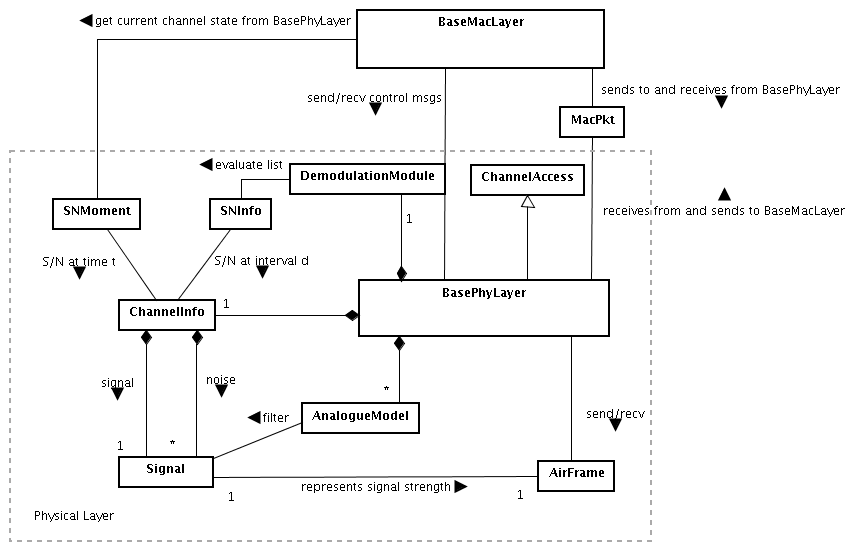
\includegraphics[width=21cm]{modelling/class_diagram.png}
 \caption{class graph}
 \label{fig: classgraph}
\end{figure}
\end{landscape} 

\subsection{The \h{\bp} interface}

In this section we focus on how one is able to communicate with the 
\h{\bp}, i.e. especially the \h{\bm} which is connected to the \h{\bp}
in three ways:

\begin{enumerate}
 \item OMNeT-channel for data messages
 \item OMNeT-channel for control messages
 \item a reference to \h{\bp}.
\end{enumerate} 

The \underline{data channel} is used to send and receive\req{packetFromMac} MacPkts to and
from the \h{\bp}. An appropriate ControlInfo is attached to the packet by the sending layer. \saf{MacToPhyCtrlInfo interface}\\

The \underline{control channel} is used by the \h{\bp} to inform the \h{\bm} about
certain events\req{provactive}, like the TX\_OVER\req{txover} message 
which indicates the end of a sending transmission.

A ChannelSenseRequest can be sent over \underline{control channel} from \h{\bm} to \h{\bp}. It is handed to the Decider (several times) that attaches a ChannelState and finally sent back to \h{\bm}.
\begin{figure}[H]
 \centering
 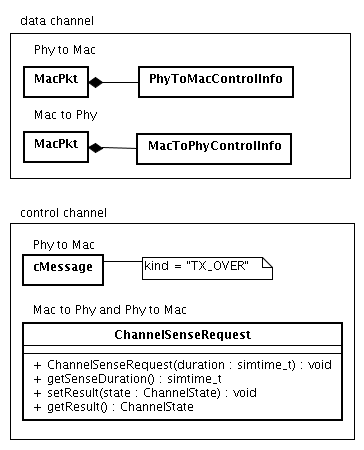
\includegraphics[width = 0.7\textwidth]{modelling/PhyMacMessages.png}
 \caption{messages sent between \h{\bp} an \h{\bm}}
 \label{fig: PhyMacMessages}
\end{figure}


The reference provides a passive way\req{provpassive} for the  \h{\bm} to  get
information about the current channel state\req{channelstate} (that is an alternative [immediate answer] to sending a ChannelSenseRequest) and to
get\req{currentmode} and set\req{switchmode} the current radiostate (RX, TX,
SLEEP).
Switching times\req{switchtimes} from one radio state to another are controlled
internally by a state machine. \saf{mode state machine}
\\

The createSignal method returns \h{\bm} a reference to a Signal at a minimum of necessary parameters, it only has to pass txPower, headerBitrate and payloadBitrate. This is the key method for \h{\bm} in order to create MacToPhyControlInfo properly.

% interface description here
\label{SignalCreation}

\begin{figure}[H]
 \centering
 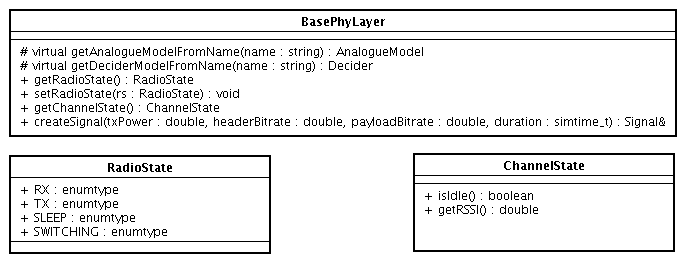
\includegraphics[width = \textwidth]{modelling/BasePhyLayer_members.png}
 \caption{BasePhyLayer interface}
 \label{fig: BasePhyLayer interface}
\end{figure}



\subsection{AnalogueModel}
%\label{AM and Signal}

%The Signal is designed one-dimensional (power-over-time) by default with a
%specified time point for start and end of the Signal. The owner is able
%to add and request values at a specific time point\req{sendInfoTXPower}.
%The Method getTimeIterator() returns an appropriate SignalTimeIterator needed
%for applying AnalogueModels to the Signal.

%\begin{quote}
%\emph{NOTE: Anyone who subclasses Signal should make shure to have a properly
%working SignalTimeIterator (subclassed) for it. The SignalTimeIterator should
%always iterate over every time stamp in each dimension. This way simple
%AnalogueModels will be able to filter the Signal independent from its
%dimension.}
%\end{quote}

%Further the Signal is set the packets bitrate over time\req{sendInfoBitrate}, 
%the Move of the Host\req{sendInfoMove}, the size of the
%packet\req{sendInfoSize} and the channel dimensions\req{sendInfoChannel} by
%\h{\bp}.
%
%\emph{See also \ref{AirFrame and Signal}.}

The AnalogueModel is at least able to filter the \emph{TX-Power over time}-Signal.\\

Information how it works on a more complex multi-dimensional Signal are
explained in section \ref{sec:signaldetail}.
 
\begin{figure}[H]
 \centering
 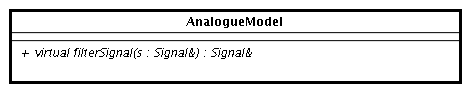
\includegraphics[width = \textwidth]{modelling/AnalogueModel_members.png}
 \caption{analogue model interface}
 \label{fig: analogue model interface}
\end{figure}
%
%The AnalogueModel offers functionality to filter a referenced
%signal\req{analogueFilter} in a specified interval\req{rcvFilterSignals} (e.g.
%preamble\req{rcvFilterPreamble}) or at a single point in time.

%Three basic AnalogueModel classes are foreseen to be plugged into Phy-Layer to
%simulate pathloss\req{analogueSimPathloss}, shadowing\req{analogueSimShadowing}
%and fading\req{analogueSimFading}.\\
%\h{\bp} is designed to apply an arbitrary number of AnalogueModels to a Signal.

% \begin{figure}[H]
%  \centering
%  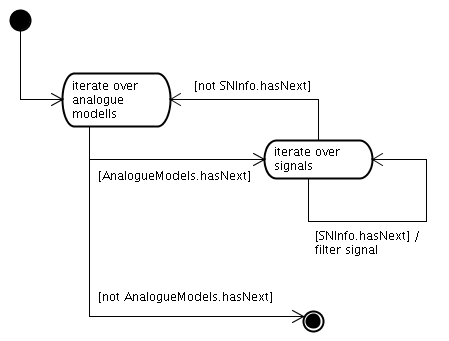
\includegraphics[width =
%0.8\textwidth]{modelling/apply_analogue_modells_detail.png}%[width=300pt]
%  \caption{application of analogue models}
%  \label{fig: application analogue models}
% \end{figure}



\subsection{ChannelInfo}

ChannelInfo keeps track of all AirFrames on the channel. It does not
differentiate between \textit{signal} and \textit{noise}. \h{\bp} is able to
add and remove references to certain AirFrames to and from ChannelInfo.\\
ChannelInfo can return a vector of Signals (references) that intersect with a
given time interval.

\begin{figure}[H]
 \centering
 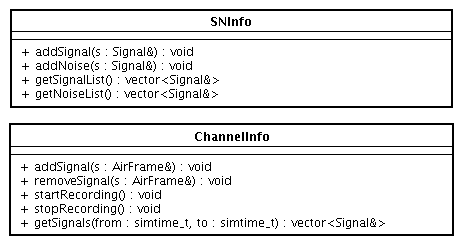
\includegraphics[width = \textwidth]{modelling/ChannelInfo_members.png}
 \caption{channel details}
 \label{fig: channel details}
\end{figure}
